\DocumentMetadata{}
\documentclass[sigconf,review]{acmart}

\makeatletter
\def\mdseries@tt{m}
\makeatother

\ifdefined\pdfoutput
\pdfoutput=1
\fi

\usepackage{amsmath}
\usepackage{amsfonts}
\usepackage{graphicx}
\usepackage{booktabs}
\usepackage{array}
\usepackage{url}
\usepackage{listings}
\usepackage{xcolor}
\usepackage{caption}
\usepackage{subcaption}
\usepackage{float}
\usepackage{geometry}
\usepackage{algorithm}
\usepackage{algorithmic}
\usepackage{multirow}
\usepackage{mdframed}
\usepackage{xstring}
\usepackage{pifont}
\usepackage[UTF8,fontset=none]{ctex}

\setCJKmainfont{Hiragino Sans GB}
\setCJKsansfont{Hiragino Sans GB}
\setCJKmonofont{Hiragino Sans GB}
\makeatletter
\let\ACM@origbaselinestretch\baselinestretch
\makeatother
\renewcommand{\abstractname}{摘要}
\renewcommand{\figurename}{图}
\renewcommand{\tablename}{表}

\usepackage{tikz}
\definecolor{GoodGreen}{RGB}{0,139,69}
\definecolor{BadRed}{RGB}{204,0,0}

\newcommand{\impact}[2]{%
  \IfStrEq{#2}{red}{%
    \textcolor{BadRed}{\textbf{#1}}%
  }{%
    \IfStrEq{#2}{green}{%
      \textcolor{GoodGreen}{\textbf{#1}}%
    }{%
      \textbf{#1}%
    }%
  }%
}

\geometry{margin=1in}

\lstset{
    basicstyle=\ttfamily\scriptsize,
    breaklines=true,
    frame=single,
    backgroundcolor=\color{gray!10},
    keywordstyle=\color{blue},
    commentstyle=\color{green!60!black},
    stringstyle=\color{red},
    showstringspaces=false,
    captionpos=b
}

\begin{document}
\sloppy
\title[Terminus-4B]{Terminus-4B：小模型能否在智能体执行任务中替代前沿 LLM？}

\author{Spandan Garg}
\email{spgarg@microsoft.com}
\affiliation{%
  \institution{Microsoft}
  \country{USA}
}
\author{Vikram Nitin}
\email{vikramnitin@microsoft.com}
\affiliation{%
  \institution{Microsoft}
  \country{USA}
}
\author{Yufan Huang}
\email{yufanhuang@microsoft.com}
\affiliation{%
  \institution{Microsoft}
  \country{USA}
}

\date{}

\begin{abstract}
现代编码智能体日益将专门子任务委派给子智能体。子智能体是更小、更聚焦的智能体循环，负责搜索、调试或终端执行等狭窄职责。这种架构通过将冗长输出（例如构建日志、测试结果等）隔离在子智能体上下文中，保持主智能体的上下文窗口整洁。通常，智能体会为这类子任务使用前沿模型。本文研究：经过微调的小语言模型（SLM）能否在智能体式终端执行任务上达到与前沿模型相当的性能。我们提出 Terminus-4B：这是一个面向该任务的 Qwen3-4B 后训练模型，通过监督微调（SFT）和强化学习（RL）获得，RL 采用基于评分量表的 LLM-as-a-Judge 奖励。在覆盖多种前沿模型、训练消融和主智能体配置的大规模评估中，我们发现，相比不使用子智能体的基线，Terminus-4B 在 SWE-Bench Pro 和我们的内部 SWE-Bench C\# 等测试基准上不损害智能体性能的同时，能够将\textbf{主智能体的词元用量最高降低约 $\sim$30\%}。该内部基准往往包含冗长的执行任务。此外，Terminus-4B 改善了多项关键指标，表明主智能体更依赖子智能体输出，也更少自行执行终端任务。我们的模型不仅弥合了原始 Qwen 模型与 Claude Sonnet / Opus / GPT-5.3-Codex 等前沿模型之间的差距，而且常常超过它们的表现。
\end{abstract}

\maketitle

\thispagestyle{empty}
\pagestyle{plain}

\section{引言}
近年来，编码智能体~\cite{vscode_2025, wang2024opendevinopenplatformai, claude_code_2024, sweagent}在软件工程任务上不断进步，覆盖从编写测试到解决复杂仓库级 GitHub 问题的工作流。这些工作流的关键组成部分是终端执行，即运行构建、安装依赖、执行诊断测试以复现问题并验证修复的过程。尽管不可或缺，这些任务会用终端输出淹没智能体的上下文窗口。

一次冗长测试就可能产生数万个词元，从而挤占智能体为后续决策所需的代码上下文、编辑与规划空间。随着轨迹增长，问题会不断累积：每一份新增命令输出都会进一步挤占上下文窗口，限制智能体在触达词元窗口上限前能够执行的真实问题求解步骤。在实践中，终端输出常是编码智能体轨迹中最大的上下文消耗来源。我们认为，让智能体在自身上下文中直接运行命令并吸收完整输出的执行方式过于原始，是当今编码智能体设计中的重大低效之处。主智能体从这些终端执行中所需的信息往往只是对过程的简明摘要，例如表示错误的一行文字或最后的一个表，而不是 shell 命令的完整原始输出。

为缓解 LLM 的上下文限制，流行编码智能体越来越多地采用子智能体架构。智能体不在主智能体循环中完成昂贵任务，而是将其委派给专门子智能体。子智能体依据给定输入独立完成任务，并以主智能体预期的格式返回输出，从而吸收中间步骤带来的上下文开销。这一模式已成功应用于搜索~\cite{claude_code_2024}、调试~\cite{debug2fix}等任务。我们认为，终端执行非常适合采用这一模式。

尽管适配性显而易见，将子智能体模式用于终端执行仍面临挑战。子智能体必须能够处理跨越多种语言的不同仓库，正确解释错误并决定后续操作，妥善处理超时等。更重要的是，它必须生成有效的最终摘要，因为那是主智能体了解子智能体工作过程的唯一窗口。产生模糊摘要（例如\textit{“构建失败了。”}）或幻觉输出的子智能体甚至比没有子智能体更糟：主智能体不仅需要重复工作，还可能被错误子智能体误导。通常，子智能体依赖前沿模型，以获得对不同任务的适应能力。鉴于本任务范围狭窄，我们认为使用昂贵的前沿 LLM 属于过度配置，更小的模型也应能够胜任。

在本文中，我们通过向既有智能体加入一个\textit{执行子智能体}，将子智能体模式应用于终端执行。该子智能体仅获得一个\textit{终端}工具，受到轮数上限约束，并使用引导其返回结构化摘要的定向系统提示。主智能体只需一个简单查询即可将任务委派给该子智能体。为避免使用昂贵的前沿 LLM，我们提出 Terminus-4B：一个专门为智能体式终端执行后训练的 Qwen3-4B~\cite{qwen}模型。我们采用两阶段训练流水线：先在内部使用遥测数据收集的轨迹上进行监督微调（SFT），随后在从 GitHub 问题整理的数据上，使用组相对策略优化（GRPO）~\cite{grpo}进行强化学习（RL），并采用新颖的子智能体训练流水线和基于评分量表的 LLM-as-a-Judge 奖励~\cite{llmjudge, rubric}。该流水线能够将子智能体任务与主智能体隔离，确保每个 rollout 从相同问题开始，同时将主智能体在 rollout 中的职责降至最低，实现低成本训练。奖励函数沿着多个质量维度与失败模式，将候选 rollout 与参考轨迹进行评分比较，为该任务提供丰富的多维训练信号。本文贡献如下：

\begin{itemize}
    \item \textbf{执行子智能体与 Terminus-4B。}我们在生产级编码智能体框架中设计并集成执行子智能体。结合执行子智能体和自定义微调的 Terminus-4B 模型，在 SWE-Bench Pro 与内部 SWE-Bench C\# 等高难度编码基准上保持智能体性能的同时，词元用量最高可降低约 $\sim$30\%。
    \item \textbf{子智能体训练框架。}我们提出一种新颖的后训练框架，将子智能体模型训练与主智能体循环解耦。该框架以极低的前沿 LLM 依赖实现快速、低成本的 rollout；在 rollout 中，甚至可以使用原始 Qwen3-4B 本身作为主智能体。
    \item \textbf{任务建模与奖励设计。}我们提出基于评分量表的多维 LLM-as-a-Judge 奖励，将 rollout 与参考轨迹沿质量和失败维度进行比较，为传统结果式奖励~\cite{instructgpt}难以直接适用的任务提供丰富训练信号。
    \item \textbf{全面评估。}我们使用 SWE-Bench Pro 和内部基准 SWE-Bench C\#，对执行子智能体设计和模型训练进行广泛消融，衡量修复率、词元效率和行为信号。我们进一步从主智能体视角，对子智能体响应进行五维 LLM 评审。在评估中，Terminus-4B 作为执行子智能体能够匹配或超过前沿模型的性能。
\end{itemize}

\section{背景与相关工作}
我们的工作与编码智能体领域多条研究线索相交并加以扩展，包括多智能体 / 子智能体架构、面向智能体工作负载的小语言模型、多轮 LLM 智能体的强化学习，以及 LLM 评审 / 基于评分量表的奖励设计。下文分别讨论。

\subsection{多智能体与子智能体架构}
将复杂任务分解给多个智能体已得到广泛研究。AutoGen~\cite{autogen}提供灵活的智能体间对话框架。MetaGPT~\cite{metagpt}、ChatDev~\cite{chatdev}等工作探索了多智能体之间基于角色的协作。He 等人~\cite{hesurvey}系统回顾了面向软件工程的 LLM 多智能体系统，梳理了这些方法当前的能力与局限。Anthropic 的多智能体研究系统~\cite{anthropicmultiagent}采用编排器--工作器模式：主导智能体将任务委派给在隔离上下文中运行的专门子智能体。Claude Code~\cite{claude_code_2024}进一步将该模式形式化为子智能体，内置通用和规划子智能体，并支持编写自定义子智能体。我们的执行子智能体遵循同一编排器--工作器模式，但专门处理编码智能体中的终端执行任务；此类任务中冗长工具输出尤为常见。

\subsection{面向智能体任务的小语言模型}
越来越多的研究指出，小语言模型是智能体 AI 未来的关键~\cite{slmfuture}。这些研究认为，大量智能体调用都是重复任务，SLM 不仅足以应对，而且比前沿 LLM 便宜 10--30 倍。Qwen3 系列~\cite{qwen}是强大的开放权重 SLM 家族，原生具备工具调用能力；越来越多研究表明，合适的后训练~\cite{deepseekr1, dangreason}能够使其在聚焦任务上获得有竞争力的结果。Terminus-4B 将这些经验和原则应用到终端执行这一目标明确却影响重大的任务上。

\subsection{终端任务与执行智能体}
与我们领域最接近的工作之一是 TerminalBench~\cite{terminalbench}。该基准在沙箱 Docker 环境中提供真实的命令行任务，发现前沿 LLM 解决的任务仍不足 65\%，而小模型仅约 15\%。近期编码智能体训练工作~\cite{qwencodernext, skyrlagent}明确将 Terminal-Bench 作为分布外任务评估，以考察 LLM 是否可泛化到此类任务。与我们工作更相关的是 Gandhi 等人~\cite{endlessterminals}：他们程序化生成终端任务，并使用原始 PPO 训练小模型执行终端操作。我们的不同之处在于，我们在从 GitHub 问题挖掘的任务上，利用新颖的基于评分量表的奖励设计进行训练，并将终端执行视作被委派的子智能体任务，目标是降低主智能体的词元用量。据我们所知，先前工作将终端执行视作主智能体的一项能力，而非可委派给运行微调小模型的专门子智能体的任务。本文填补了这一空白。

\subsection{长程任务的上下文管理}
随着 LLM 与智能体能力增长，其轨迹也变得更长，上下文管理成为智能体设计中的重要议题。长上下文会推高成本，并因分散对轨迹中任务相关词元的注意力而削弱推理能力。Focus~\cite{focus}提出一种智能体，使其自主决定何时将关键学习内容整合到持久块中，并主动裁剪智能体交互历史。Sun 等人提出 Context Folding~\cite{contextfolding}，允许智能体分支出子轨迹处理子任务，再将其折叠回主轨迹。Memex(RL)~\cite{memex}以精炼的结构化摘要和稳定索引提供紧凑上下文表示；SWE-ContextBench~\cite{swecontextbench}则明确评估摘要上下文与原始上下文如何影响编码智能体能力。我们的子智能体方法与这些工作互补：它不压缩上下文，而是让执行子智能体在独立智能体循环中运行冗长终端命令，阻止其输出进入主智能体上下文，只返回结构化摘要。

\section{动机示例}
本节通过一个真实案例说明方法优势。图~\ref{motivating_example}展示了在 Serilog C\# 仓库中解决同一任务（\texttt{serilog/serilog \#2053}）的两条智能体轨迹。该问题要求智能体新增一组批处理 API。由于这是全新功能，智能体必须构建解决方案、运行单元测试、识别失败，并应用必要修复以消除构建 / 测试错误。

比较使用和不使用子智能体的轨迹，可看到显著不同的结果。对于基线智能体，每条终端命令都会将完整原始输出直接返回其上下文窗口。整个轨迹中，主智能体直接调用终端 18 次，其中很多只是略有变化的重复调用：智能体尝试不同的 \texttt{grep} 和 \texttt{tail} 过滤器组合，从冗长的构建和测试日志中提取相关信息。例如：

\begin{lstlisting}[basicstyle=\ttfamily\tiny]
$ dotnet test ... 2>&1 | tail -40
$ dotnet test ... 2>&1 | grep -E "passed|failed|error"
$ dotnet test ... 2>&1 | grep -A 10 "Error Message"
$ dotnet test ... 2>&1 | grep -E "passed|failed|Error Message|Assert"
$ dotnet test ... 2>&1 | tail -20
...
\end{lstlisting}

每次调用都会向上下文加入新的原始输出，并在后续每一轮作为 LLM 的输入上下文传递。至轨迹结束，该智能体在 40 轮中消耗了 \textbf{2.46M} 个主智能体词元，其中大部分上下文来自终端输出。

在子智能体配置中，主智能体以单一查询将相同任务委派给执行子智能体（使用经过 RL 训练的 Terminus-4B）：\texttt{“Run the build, then the unit and approval tests, and report pass/fail counts with error details”}。子智能体在自身上下文中共执行 9 条命令，并返回如下最终答案：

\begin{lstlisting}[basicstyle=\ttfamily\tiny]
<final_answer>
Command: dotnet build /testbed/Serilog.sln
Summary: Build succeeded. 9 warnings, 0 errors.

Command: dotnet test .../Serilog.Tests.csproj
Summary: All 769 tests passed, 0 failed, 0 skipped.

Command: dotnet test .../Serilog.ApprovalTests.csproj
Summary: Test Run Failed - 1 failed.
  Error: Serilog.received.txt does not match Serilog.approved.txt.
  The diff shows new API surface in LoggerAuditSinkConfiguration.
  To fix: update the approved snapshot file.
</final_answer>
\end{lstlisting}

主智能体接收的不是完整原始终端输出，而是每次仅约 200 个词元的摘要，能够立即定位导致测试失败的根本问题。总体而言，该轨迹在 32 轮中仅消耗 740k 个主智能体词元，显著少于基线。此外，由于子智能体使用 Terminus-4B，所消耗词元的成本只占主智能体词元成本的一小部分。这一对比突出了该子智能体的必要性。

\begin{figure*}
    \centering
    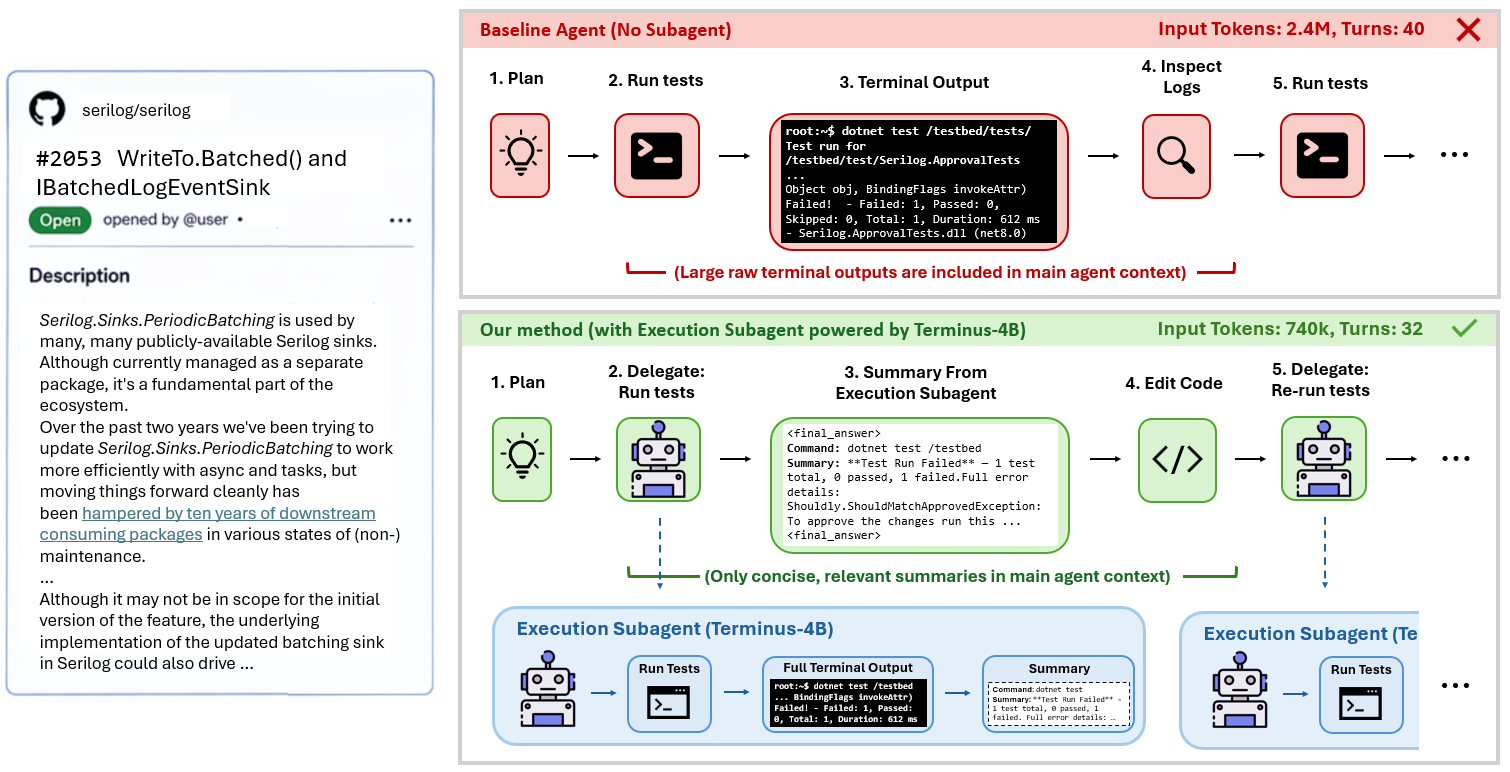
\includegraphics[width=0.95\linewidth]{figures/comparison_issue.png}
    \caption{Serilog 仓库真实问题的两条对比智能体轨迹，分别使用和不使用执行子智能体。没有子智能体时（上），主智能体必须直接调用终端命令、处理冗长构建与测试输出，并额外花费轮次解释结果，因而消耗显著更多词元和轮次。使用子智能体时（下），终端执行任务被委派给子智能体；它吸收原始输出，并仅以预定义格式的简洁最终答案返回关键发现。主智能体无需处理冗长终端输出，从而保留上下文窗口。}
    \label{motivating_example}
\end{figure*}

\section{方法}
本节介绍执行子智能体的设计、它如何集成到既有编码智能体中，以及用于得到 Terminus-4B 的后训练流水线。图~\ref{train}概述了我们的方法。首先定义子智能体：

\textbf{子智能体：}由父（或“主”）智能体调用、用于处理专门子任务的次级 LLM 智能体循环。主智能体解决广泛任务，而子智能体处理更窄、通常也更简单的任务集合。与主智能体相似，子智能体拥有自己的系统提示、上下文窗口和工具集，用来实现主智能体委派的目标。

\subsection{执行子智能体}
\textit{执行子智能体}是一种专门按顺序生成并执行终端命令、向主智能体返回结果结构化摘要的子智能体。它以一个简单工具的形式暴露给主智能体，只接收以下两个参数：
\begin{itemize}
   \item \textbf{查询（必需）：}执行任务的自然语言描述，即要运行哪些命令、需要报告哪些信息。例如：\textit{“运行测试套件，并报告失败的测试及其错误消息。”}
   \item \textbf{描述（必需）：}当子智能体运行时，在 UI 中展示给用户的简短说明。
\end{itemize}

子智能体返回结构化响应，其中包含每条已运行命令的摘要、结果及所有相关输出（错误消息、测试计数、构建状态），并使用 XML 风格的 \texttt{<final\_answer>} 标签界定。这个简单的问答接口将主智能体与原始终端输出的冗长性隔离开来。主智能体可以灵活描述希望运行和返回的内容，子智能体负责决定如何达成。

\subsubsection{工具与轮数限制}
执行子智能体只有一个工具：\texttt{Terminal}。该工具接收一条 shell 命令、执行模式（同步或异步）和以毫秒为单位的超时，返回截断到 60KB 的 shell 命令输出。这正是提供给主智能体运行终端命令的工具。此外，我们还限制子智能体每轮只能调用该工具一次，即不支持并行工具调用，使用同步模式并指定超时，同时受可配置轮数上限约束，默认上限为 10。若子智能体尚未自行退出便达到轮数上限，我们会注入一条用户消息（\textit{“OK, your allotted iterations are finished. Show the \texttt{<final\_answer>}.”}），促使其给出最终答案。

这些约束简化了设计，也使子智能体保持聚焦且可预测。子智能体没有读取文件、编辑代码或其他任何工具，只能运行终端命令。正是这一狭窄范围使该任务适合由更小的微调模型完成。

\subsubsection{系统提示}
图~\ref{exec_system_prompt}展示执行子智能体所用的系统提示。该提示指示模型：1）运行终端命令以完成委派任务，并按需调整命令；2）遵守 \texttt{Terminal} 工具使用规则，例如同步模式、显式超时和禁止并行调用；3）返回包含逐命令摘要的 \texttt{<final\_answer>}，其中列出所运行命令和结果的简洁说明。提示还包含一个两步交互示例（失败的 \texttt{make} 命令，随后是成功的 \texttt{cmake \&\& make}）及对应格式化的 \texttt{<final\_answer>}。该示例帮助模型理解预期行为和输出结构。

\subsubsection{主智能体集成}
执行子智能体被注册为主智能体可用工具之一，与 \texttt{ReadFile}、\texttt{Grep}、\texttt{Edit} 等工具并列。我们还扩展主智能体系统提示（图~\ref{main_prompt_diff}），说明何时以及如何调用执行子智能体。

我们还支持独立配置驱动子智能体的模型。默认配置使用与主智能体相同的前沿模型（例如 Claude Sonnet 4.6、GPT-5.3-Codex 等）。尽管这可以产生高质量轨迹和最终响应，却极其浪费：子智能体的运行命令和摘要输出任务既冗长又消耗大量词元，但相较主智能体的开放式规划和代码编辑，它的范围狭窄且结构清晰。因此，使用前沿模型属于过度配置。下一节将说明如何训练 Terminus-4B：一个专门针对该任务后训练的 Qwen3-4B 模型，用于替代子智能体中的前沿模型，同时保持、在某些情况下甚至改善整体智能体性能。

\begin{figure}
    \centering
    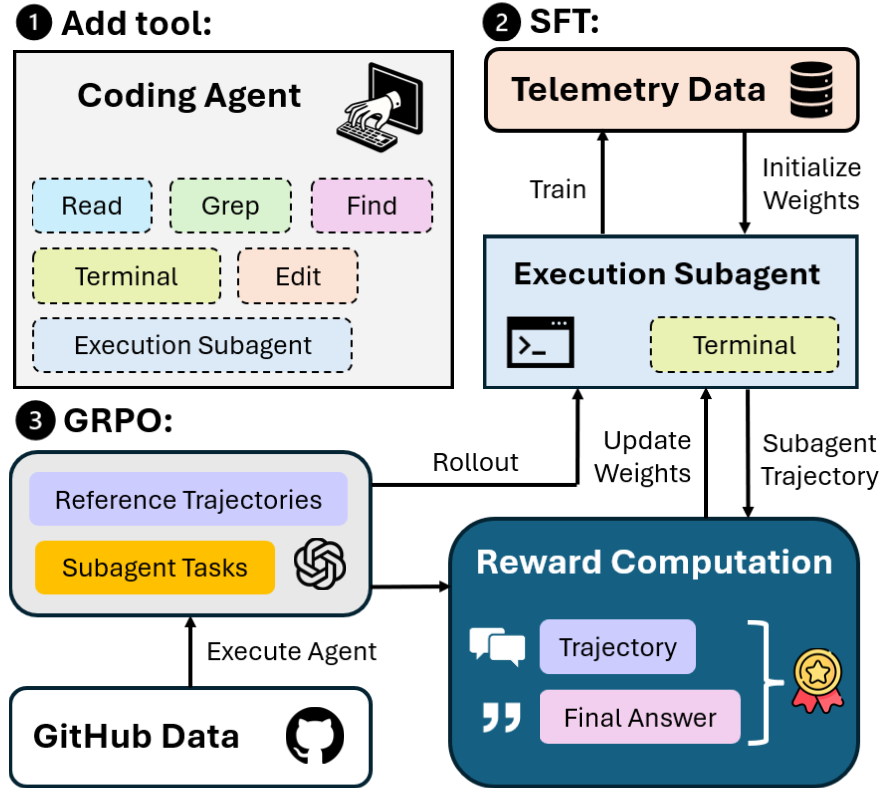
\includegraphics[width=0.99\linewidth]{figures/post_train_pipeline.png}
    \caption{Terminus-4B 训练流水线。\ding{182} 首先将执行子智能体作为工具集成到主智能体框架中。\ding{183} 随后进行 SFT，在遥测数据中的专家轨迹上微调基础 Qwen3-4B 模型。\ding{184} 最后在 GitHub 样本上用 GRPO 进行进一步 RL 训练；rollout 由基于评分量表的 LLM-as-a-Judge 奖励、相对于前沿 LLM 生成的参考轨迹进行评分。}
    \label{train}
\end{figure}

\begin{figure}[t]
\centering
\fbox{%
\begin{minipage}{0.92\columnwidth}
\scriptsize
\ttfamily
\setlength{\parskip}{1pt}
\noindent 你是一名 AI 编码研究助手，负责运行终端命令以完成一个小型、以执行为中心的任务。\\[3pt]
你将获得任务描述，也可能得到一些建议命令，但可按需调整。\\[3pt]
\textbf{run\_in\_terminal 的规则：}\\
- 始终使用 mode="sync".\\
- 必须包含以毫秒计的 "timeout"（短任务 30000，构建任务 120000）。\\
- 每轮只能调用 run\_in\_terminal 一次。\\
- 用 --yes、-y 或 \texttt{yes} 自动确认提示。\\[3pt]
\textbf{输出格式（必需）}\\
完成后，只返回一个 \textless final\_answer\textgreater{} 标签，其中给出每条命令的紧凑摘要：\\[2pt]
\phantom{x}\textless final\_answer\textgreater\\
\phantom{x}Command: cmake . \&\& make\\
\phantom{x}Summary: Build unsuccessful. Excerpt: ...\\
\phantom{x}\textless/final\_answer\textgreater\\[3pt]
\textbf{可用工具}\\
- run\_in\_terminal: 执行 shell 命令
\end{minipage}%
}
\caption{执行子智能体的系统提示。子智能体被限制为单一工具（\texttt{Terminal}），只能运行同步命令，并且必须返回结构化的 \texttt{\textless final\_answer\textgreater} 摘要。}
\label{exec_system_prompt}
\end{figure}

\begin{figure}[t]
\centering
\fbox{%
\begin{minipage}{0.92\columnwidth}
\scriptsize
\ttfamily
\setlength{\parskip}{1pt}
\noindent 你是一名高度成熟的自动化编码智能体，拥有跨多种编程语言和框架的专家级知识……\\[4pt]
\noindent 自定义工具（Grep、FileSearch、ReadFile、ListDir）已针对智能体界面优化。
优先使用它们，而不是终端命令……\\[5pt]
\colorbox{green!20}{\parbox{0.97\columnwidth}{\textbf{== 使用 ExecutionSubagent ==}\\[2pt]
对于大多数执行任务和终端命令，使用 \texttt{ExecutionSubagent} 来运行命令并获取相关输出片段，而不是直接使用 \texttt{Terminal}。仅当你希望获得一条命令未经截断的完整输出时，才在少数场景使用 \texttt{Terminal}。\\[3pt]
不要并行调用多次 \texttt{ExecutionSubagent}。应调用一个子智能体并等待其响应，再运行下一条命令。}}\\[5pt]
\noindent 调用需要文件路径的工具时，始终使用绝对文件路径……
\end{minipage}%
}
\caption{以绿色展示的、添加到主智能体系统提示中的指令。我们要求主智能体将终端执行委派给执行子智能体。}
\label{main_prompt_diff}
\end{figure}

\section{后训练流水线}
为训练 Terminus-4B，我们执行图~\ref{train}所示的两阶段后训练流水线。首先在由专家轨迹构成的内部遥测数据上进行监督微调（SFT）；随后在精心筛选的 GitHub 问题数据集上，采用组相对策略优化（GRPO）进行强化学习（RL），以与前沿 LLM 生成的专家轨迹比较 rollout 的奖励进行训练。

\subsubsection{数据收集}
\label{data}
我们构建了一个包含约 $\sim$3200 个执行任务的训练数据集，覆盖 GitHub 上多个编程语言和项目。起初有一个约 $\sim$10k 个样本的候选池，来自 2{,}144 个仓库和 5 种语言（TypeScript、C\#、Java、JavaScript、Python）；我们确认其中每个仓库均可构建。对于每个样本，仓库会在开发者修复前的提交处检出，并置于 Docker 容器中，项目依赖已预先安装。

随后，我们在约 2k 个样本上，以前沿 LLM 作为主智能体并启用执行子智能体来运行智能体。每次运行中，主智能体都会被提示使用执行子智能体，并在轨迹的不同位置自主决定调用它。我们从所得轨迹中提取每次子智能体调用，捕获：1）主智能体发出的\textit{查询}；2）包含所有 \texttt{Terminal} 调用、命令输出、退出码及返回主智能体的 \texttt{<final\_answer>} 的完整子智能体轨迹；3）子智能体被调用前的仓库状态。随着后文展开，这些字段的必要性将变得清晰。

\begin{table}[t]
\centering
\caption{按语言划分的收集任务分布。}
\label{dataset_languages}
\small
\begin{tabular}{lr}
\toprule
\textbf{语言} & \textbf{数量} \\
\midrule
TypeScript & 1{,}011 (36.5\%) \\
C\# & 770 (27.8\%) \\
Java & 725 (26.2\%) \\
JavaScript & 196 (7.1\%) \\
Python & 65 (2.3\%) \\
\midrule
\end{tabular}
\end{table}

所得轨迹包含来自 730 个仓库的 3{,}009 次独特执行子智能体调用。我们将这些轨迹视为金标准\textit{参考轨迹}，后续在 RL 中用它们对 rollout 评分。表~\ref{dataset_languages}展示所收集问题的语言分布。可以看到，受数据集构成影响，TypeScript 和 C\# 占主导；但数据仍覆盖 5 种语言的 720 个仓库，以及使用 \texttt{npm}、\texttt{dotnet}、\texttt{mvn}、\texttt{gradle}、\texttt{pip} 等多样构建系统。表~\ref{dataset_task_types}展示数据中任务种类（由简单提示分类）。其中大多数是测试执行、错误诊断或构建任务，这符合预期：运行测试通常需要先构建项目，而编译错误或构建失败通常需要进行错误诊断。

\begin{table}[t]
\centering
\caption{收集执行任务集合中包含的任务类型。}
\label{dataset_task_types}
\small
\begin{tabular}{lr}
\toprule
\textbf{任务类型（可多选）} & \textbf{数量} \\
\midrule
测试执行 & 2{,}692 (97.3\%) \\
构建 / 编译 & 969 (35.0\%) \\
错误诊断 & 2{,}166 (78.3\%) \\
依赖项 & 106 (3.8\%) \\
\bottomrule
\end{tabular}
\end{table}

\subsubsection{阶段 I：监督微调}
在进行 RL 前，我们使用从内部使用遥测数据收集的专家轨迹，对基础 Qwen3-4B 模型进行监督微调以实现冷启动。当生产环境中执行子智能体由前沿模型运行时，每次调用都会产生一个完整多轮轨迹：系统提示、用户查询、含终端输出的工具调用以及最终的 \texttt{<final\_answer>}。我们提取这些轨迹作为 SFT 数据。为防止数据泄漏，我们还确保 SFT 与 RL 数据集来自互不重叠的仓库集合。

我们采用标准语言建模损失及损失掩码：仅对助手词元计算梯度，即工具调用和最终答案，而不对系统提示、用户消息和工具输出计算梯度：

\begin{equation}
\mathcal{L}_{\text{SFT}} = -\sum_{t \in \mathcal{A}} \log p_\theta(x_t \mid x_{<t})
\label{eq:sft}
\end{equation}

\noindent 其中，$\mathcal{A}$ 表示经过掩码后、词元序列中带有助手响应的位置集合。我们仅进行两个 epoch 的轻量训练。该阶段使模型学习任务机制，包括如何使用终端工具、解释输出、以及写出有用的最终响应，为 RL 训练提供强有力的初始化。

\subsubsection{阶段 II：强化学习}
从 SFT 检查点出发，我们在第~\ref{data}节收集的 2.7k 个执行任务上，使用组相对策略优化（GRPO）~\cite{grpo}进行在线 RL。虽然 SFT 使模型掌握总体任务形态，却未必能针对执行子智能体最关键的性质进行优化，例如带有充分细节的准确最终答案。使用精心设计的奖励进行 RL，可以直接塑造此类行为；但首先需要说明如何大规模生成 rollout。

\paragraph{子智能体 rollout 框架。}
RL 训练智能体的一项关键挑战是：每个 rollout 都需要端到端执行，且必须从同一初始状态开始（即相同初始提示、问题、仓库状态等）。若训练的是主智能体，这一点较易实现；但对于子智能体，要在 rollout 之间保持这种一致性则略复杂。

我们通过在训练中将主智能体与子智能体解耦来解决该问题。每个训练样本均带有数据收集阶段（第~\ref{data}节）取得的预生成查询（即执行子智能体的输入）和仓库状态。生成 rollout 时，我们使用轻量的透传模型（Qwen3-4B Instruct-2507）作为主智能体；该模型仅配置一个工具（\texttt{Execution Subagent}）及 1 轮上限。这确保主智能体在其第一轮也是唯一一轮中，确定性地将预生成查询转发给子智能体。我们将每个查询封装为如下简单指令：
\begin{center}
\small
\fbox{\parbox{0.78\columnwidth}{\ttfamily\scriptsize
请以此查询调用 Execution Subagent。你必须\\
仅使用这一\textbf{精确}查询调用 Execution Subagent。\\[4pt]
<query>\\
在 /testbed 中运行 \textasciigrave dotnet build PdfSharpCore.sln\textasciigrave{} 以检查\\
编译错误，然后运行 \textasciigrave dotnet test\\
PdfSharpCore.Test.csproj\textasciigrave{} 并报告所有测试失败。\\
</query>
}}
\end{center}

需要指出的是，我们确保主智能体行为确定性，但子智能体的行为完全由正在训练的策略模型决定，并可运行完整轨迹；之后主智能体轨迹即告结束。如此解耦的一项关键优势是，能够消除使用前沿 LLM 作为主智能体的成本，实现快速且低廉的 rollout。

每个 rollout 都在 Docker 容器中执行。容器包含经过必要修改的智能体、在正确提交处检出的目标仓库、构建项目和运行智能体所需的依赖。在 rollout 前，我们还应用代码补丁，确保仓库状态与参考轨迹中调用执行子智能体前的状态相匹配。补丁是否为空取决于参考轨迹中调用子智能体的时机。最后，我们使用 Azure Container Apps（ACA）编排并行 rollout。

\paragraph{奖励设计。}
要使 RL 在 SFT 基础上继续改进，有效的奖励设计至关重要。执行子智能体 rollout 的质量很难评判，因为许多环节都可能出错。例如，子智能体可能执行正确命令，却产生模糊摘要；也可能写出细致摘要，但其中含有幻觉信息。进一步而言，直接比较原始轨迹也很困难，因为两次有效运行可能使用完全不同的命令并产生不同输出。

我们设计了基于评分量表的 LLM-as-a-Judge 奖励，将奖励拆为对应两项主要关切的两个子部分：\textit{子智能体是否执行了正确命令？}以及\textit{最终答案对主智能体工作流有多大帮助？}第二部分尤其重要，因为最终摘要是主智能体了解子智能体行为的\textit{唯一}窗口。

\begin{figure}[t]
\centering
\fbox{%
\begin{minipage}{0.92\columnwidth}
\scriptsize
\ttfamily
\setlength{\parskip}{1pt}
\noindent\textbf{系统：}你是一名有帮助的助手，负责创建执行计划，概括 AI 智能体运行终端命令时做了什么。你的计划应遵循以下模板：\\[3pt]
\textbf{执行计划}\\[2pt]
\textbf{任务结果：} [成功 / 失败 / 部分完成。一句话。]\\[2pt]
\textbf{已执行命令：} [针对每条命令：运行了什么、为什么运行、发生了什么。包含退出码。]\\[2pt]
\textbf{关键发现：} [错误消息、版本号、测试计数、构建产物等。]\\[2pt]
\textbf{错误恢复：} [如何处理失败？进行了哪些调整？]\\[2pt]
\textbf{最终状态：} [完成了什么？]\\[6pt]
\textbf{用户：}\\
\#\# 任务查询\\
\{query\}\\[2pt]
\#\# 轨迹数据\\
\#\#\# 命令 1: \textasciigrave cmake . \&\& make\textasciigrave\\
退出码: 0\\
输出: \textit{（截断的开头 + 结尾）}\\[2pt]
\#\#\# 命令 2: \textasciigrave make test\textasciigrave\\
退出码: 1\\
输出: \textit{（截断的开头 + 结尾）}\\[2pt]
\#\# 返回给父智能体的最终答案\\
\{final\_answer\}\\[2pt]
请按上述模板创建详细执行计划。
\end{minipage}%
}
\caption{使用前沿 LLM 从原始轨迹生成执行计划的提示。命令输出被截断为前 500 个和后 500 个字符，以在保持提示紧凑的同时保留关键信息（错误通常出现在末尾，配置信息常在开头）。我们用它将参考轨迹和 rollout 轨迹都转化为相应执行计划。}
\label{execution_plan_prompt}
\end{figure}

要将子智能体行为与参考结果比较，可以把完整 rollout 和参考轨迹交给 LLM；但这样成本很高。每次奖励计算都要处理一次参考轨迹，即成本为 $N$ 倍。我们不比较冗长原始轨迹，而是先用图~\ref{execution_plan_prompt}的提示，将每个 rollout 轨迹压缩为称作\textit{执行计划}的结构化摘要。我们向前沿 LLM 提供轨迹的精炼版本，其中包含全部命令。

同样的提取过程在数据收集时应用于参考轨迹，从而产生作为真值的参考执行计划。这一中间表示将轨迹标准化为可比较的格式，与具体使用的命令无关。随后，我们使用强大的前沿 LLM，沿三个组别中的 14 个评分量表维度，将候选计划与参考计划进行评分：
\begin{itemize}
    \item \textbf{执行质量：}评审器在 7 个维度评估候选计划：命令正确性、错误处理、结果准确性、关键信息提取、完整性、效率和可操作性。将这些分数平均得到 $\bar{s}_{\text{pos}}$。
    \item \textbf{失败模式：}评估 4 个失败模式维度：幻觉结果、遗漏错误、错误诊断和不必要命令。平均后得到 $\bar{s}_{\text{pit}}$。
    \item \textbf{最终答案质量：}评估返回主智能体的最终答案质量的 3 个维度：细节程度、事实准确性和信息量。该组专门针对 \texttt{<final\_answer>}，因为它是主智能体看到的\textit{唯一}输出。平均得到 $\bar{s}_{\text{fa}}$。
\end{itemize}

最终奖励将执行质量与最终答案质量结合：
\begin{equation}
r = (1 - \alpha)(\bar{s}_{\text{pos}} -
\bar{s}_{\text{pit}}) + \alpha \cdot
\bar{s}_{\text{fa}}
\label{eq:reward}
\end{equation}
其中 $\bar{s}_{\text{pos}}$、$\bar{s}_{\text{pit}}$ 与 $\bar{s}_{\text{fa}}$ 分别是正向、失败陷阱和最终答案维度分数的均值。我们使用 $\alpha=0.5$。

在评分量表判定前，我们还对退化 rollout 施加硬惩罚。轨迹超过 30K 词元时令 $r=-100$；缺少 \texttt{<final\_answer>} 标签时令 $r=-100$；未运行任何命令的 rollout 令 $r=-50$。我们还丢弃奖励标准差 $\sigma_G < 0.01$ 的提示组，因为所有 $G$ 个 rollout 得到几乎相同的分数时，GRPO 可学习的梯度信号可以忽略不计。

\begin{figure*}[t]
   \centering
   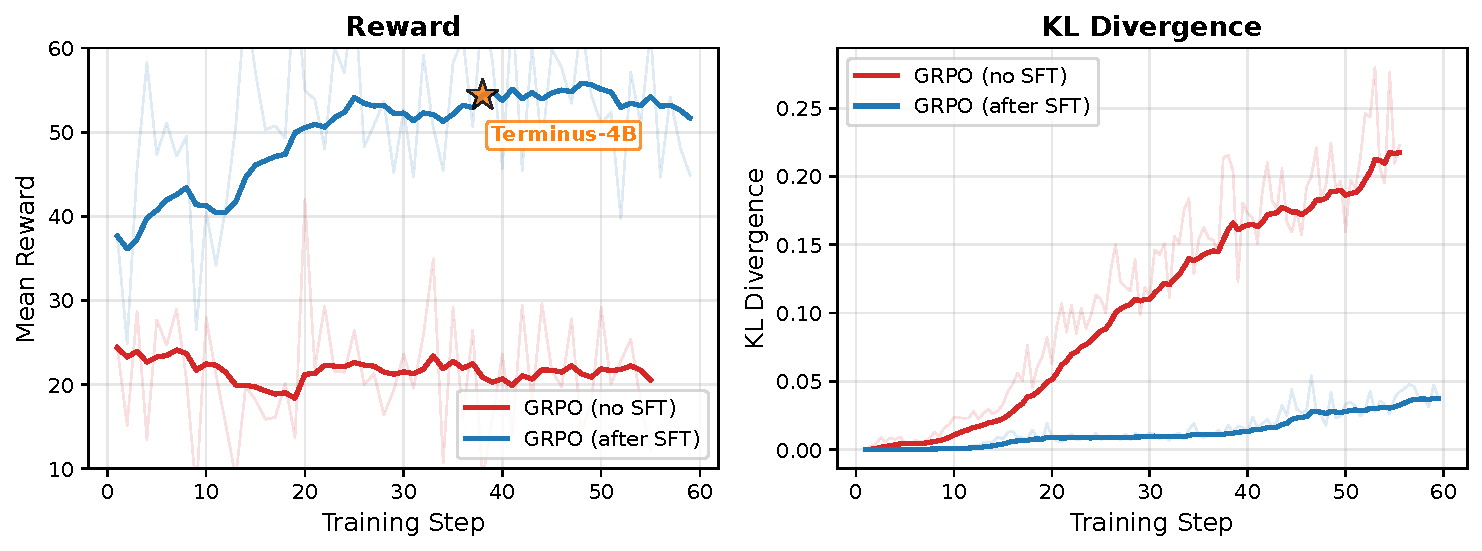
\includegraphics[width=0.9\linewidth]{figures/training_curves_fix_y.pdf}
   \caption{采用和不采用 SFT 初始化时的 GRPO 训练曲线。SFT 为 RL 训练提供强先验，使其获得更高奖励并能够学习。KL 曲线表明，训练运行保持接近参考模型（SFT 检查点）。可以清楚看到，从 SFT 检查点开始的增益。}
   \label{training_curves}
\end{figure*}

\section{实验设置}
\subsection{训练设置}
所有训练运行均使用一台配备 8 张 NVIDIA A100/H100 GPU 的单节点。推理时，我们将模型部署在 Fireworks 平台~\cite{fireworks}上。

\subsubsection{SFT 细节}
我们首先使用 Slime~\cite{slime}，基于遥测数据对 Qwen3-4B-Instruct-2507 基础模型进行全量 SFT。训练 2 个 epoch，采用 Adam 优化器（$\beta_1{=}0.9$、$\beta_2{=}0.95$），峰值学习率为 $2 \times 10^{-5}$，余弦衰减至 $2 \times 10^{-6}$，并进行 5\% 线性 warmup。全局 batch size 为 32，权重衰减为 0.01；使用动态 batching，每张 GPU 最多 8{,}192 个词元。损失只在助手词元上计算。

\subsubsection{RL 细节}
从 SFT 检查点出发，我们采用带非对称裁剪~\cite{dapo}的 GRPO 进行在线 RL，以减少过早坍塌。对于每个提示 $x$，我们采样 $G=8$ 条 rollout $\{a_i\}_{i=1}^{G} \sim \pi_{\theta_{\text{old}}}(\cdot \mid x)$，并优化以下目标：

{\fontsize{6.8pt}{10pt}\selectfont
\begin{equation}
\begin{split}
   J(\theta) = \frac{1}{G} \sum_{i=1}^{G}
   \min\!\Big(
     r_i(\theta)\,\hat{A}_i,\; \text{clip}\big(r_i(\theta),
       1{-}\epsilon_l,
       1{+}\epsilon_h\big)\hat{A}_i
   \Big) - \beta\, D_{\text{KL}}\!\big[\pi_\theta \| \pi_{\text{SFT}}\big]
   \end{split}
\end{equation}
}

\noindent 其中 $r_i(\theta)=\frac{\pi_\theta(a_i\mid x)}{\pi_{\theta_{\text{old}}}(a_i\mid x)}$ 是重要性比率，$\hat{A}_i$ 是组归一化优势。我们使用非对称裁剪阈值 $\epsilon_{\text{low}}=0.20$、$\epsilon_{\text{high}}=0.28$，为策略提高高奖励概率保留更多空间。KL 惩罚使用 $\beta=0.02$，以 SFT 检查点作为参考模型计算，从而避免相对参考模型和基础模型行为发生灾难性漂移。训练采用恒定学习率 $10^{-6}$ 和 1.0 的梯度裁剪。rollout batch size 为 16 个提示（每个提示有 $G{=}8$ 个样本），即每步产生 128 条 rollout，全局训练 batch size 为 64。奖励计算中，执行计划由前沿 LLM 生成并评分。

\subsection{评估设置}
本节说明我们对该技术进行的离线评估、所用基准及测量指标。

\subsubsection{基准}
我们在两个基准上评估方法：
\begin{itemize}
    \item \textbf{SWE-Bench Pro：}该基准~\cite{swepro}包含来自多样样本的问题，专门设计以解决 SWE-Bench~\cite{swebenchverified}面临的一些问题，覆盖多种语言和领域。我们运行完整集合中的约 $\sim$731 个样本。
    \item \textbf{SWE-Bench C\#：}这是我们的内部基准，含 150 个从 C\# 仓库收集、采用 SWE-Bench 风格构建的 GitHub 问题。解决该基准的问题需要大量项目构建 / 测试运行，因此特别适合评估本方法。
\end{itemize}

\subsubsection{消融}
给定这些基准，我们设计一组消融实验以检验两件事：1）方法的端到端智能体性能，即方法不会损害智能体解决问题的能力，也不会负面影响词元消耗等；2）子智能体输出质量，即主智能体是否真正认为子智能体输出有用。

实验使用以下子智能体配置，从不使用子智能体到希望测量性能的多种模型：
\begin{itemize}
    \item \textbf{Opus / Sonnet：}使用前沿 LLM Opus / Sonnet 作为子智能体，用于表示能力上界。
    \item \textbf{Vanilla-4B：}使用基础 Qwen3-4B-Instruct-2507 作为子智能体。
    \item \textbf{SFT-4B：}使用 SFT 后的检查点作为子智能体。
    \item \textbf{Terminus-4B：}使用 RL 后的峰值检查点作为子智能体背后的模型。
\end{itemize}

我们将这些子智能体配置与 3 个能力递增的前沿 LLM 主智能体结合：GPT-5.3-Codex、Claude Sonnet 4.6 和 Claude Opus 4.6。

\subsubsection{工具配置}
我们对不同工具配置进行消融，以隔离子智能体对智能体性能的影响：
\begin{itemize}
    \item \textbf{仅 Terminal 工具（无子智能体）：}执行子智能体完全禁用，主智能体系统提示也保持不变。这是基线。
    \item \textbf{子智能体 + Terminal 工具：}启用执行子智能体与 Terminal 工具。主智能体可选择将终端工作委派给子智能体，或直接通过 Terminal 运行。
    \item \textbf{仅子智能体（无 Terminal）：}执行子智能体是主智能体唯一可用的终端执行工具。
\end{itemize}

\begin{figure}[t]
\centering
\fbox{%
\begin{minipage}{0.92\columnwidth}
\scriptsize
\ttfamily
\setlength{\parskip}{1pt}
\noindent\textbf{系统：}你是一名严格评估者，负责评估执行子智能体响应的质量。主智能体只能看到子智能体的最终响应，无法访问中间命令或原始输出。\\[3pt]
请沿以下维度打分（0.0--1.0）：\\[2pt]
\textbf{task\_completion}：子智能体是否完整完成所要求的任务？\\
\textbf{factual\_accuracy}：响应是否有事实依据且可验证？（退出码、路径、精确错误）\\
\textbf{informativeness}：是否有足够细节使主智能体无需重跑命令即可继续？\\
\textbf{relevance}：是否聚焦于查询，没有无关内容？\\
\textbf{actionability}：主智能体能否据此确定明确的下一步？\\[4pt]
\noindent\textbf{用户：}\\
\#\# 主智能体上下文\\
系统提示（节选）：\{system\_prompt\}\\
问题陈述：\{problem\_statement\}\\
当前轨迹：\{trajectory\}\\[2pt]
\#\# 子智能体查询\\
\{subagent\_query\}\\[2pt]
\#\# 子智能体响应\\
\{subagent\_response\}\\[2pt]
\#\# 后续轨迹（之后的 \{N\} 轮）\\
\{trajectory\_after\}\\[2pt]
请使用后续轨迹评估主智能体是否有效利用该响应。
\end{minipage}%
}
\caption{LLM 评审打分提示的精简版本。评审器接收子智能体调用前后主智能体的完整上下文，并沿 5 个维度对响应评分。调用后轨迹中的后续 $N=5$ 轮能够反映该响应在实践中是否有用。}
\label{judge_prompt}
\end{figure}

\subsubsection{指标}
对于所有配置，我们使用评估 harness 的结果和智能体轨迹计算以下指标：
\begin{itemize}
    \item \textbf{解决率（\%）：}通过基准评估的样本比例。
    \item \textbf{词元用量：}智能体配置消耗的平均输入和输出主智能体 / 子智能体词元。
    \item \textbf{主智能体 Terminal 调用：}主智能体直接调用 Terminal 工具的平均次数。
    \item \textbf{子智能体后接 Terminal 调用：}每个样本中，执行子智能体后紧接着调用 Terminal 工具的平均次数。我们预计其中大量情况是主智能体因子智能体输出不够有用而不得不重做工作。
    \item \textbf{最终答案率（\%）：}返回由 \texttt{<final\_answer>} 标签界定的格式良好最终答案的子智能体调用比例。
    \item \textbf{LLM 评审得分：}为衡量子智能体最终答案的效用，我们计算 LLM 得分：LLM 获得调用子智能体前的轨迹、最终响应以及调用后 $N=5$ 个步骤，以判断结果是否真正被使用。LLM 被提示沿多个维度对最终响应评分，所用提示见图~\ref{judge_prompt}。
\end{itemize}

\section{结果}
\subsection{RL 训练}
图~\ref{training_curves}展示两种配置在训练过程中奖励和 KL 散度的变化：直接在基础 Qwen3-4B-Instruct-2507 模型上应用 GRPO（即不进行 SFT），以及从 SFT 检查点开始 GRPO。

比较奖励曲线可见，“无 SFT”运行的奖励在约 $\sim$20 处平台化，相比运行初始的基线分数没有改进；但 KL 散度迅速升至 0.2 以上，说明策略显著偏离参考模型却没有产生有意义学习。我们认为，原因是基础模型没有对任务及输出格式等形成基本理解，训练中无法偶然发现这些行为，从而不能为 GRPO 提供强化此类行为所需的梯度信号。

与此形成鲜明对比的是，从 SFT 检查点开始的 RL 在约 $\sim$37 的更高奖励起步，并稳定上升至 50 以上，而 KL 保持接近 SFT 检查点（差距在 0.05 以内）。直观而言，SFT 为模型提供了良好的任务机制起点，包括所需输出格式、Terminal 工具使用等。这些结果确认 SFT 不只是有帮助，而是训练必不可少的组成部分。我们将 RL 训练得到的模型称为\textbf{Terminus-4B}，并在消融中展示 RL 训练本身的效用。

\subsection{基准消融}
本小节讨论在评估基准上开展的不同消融。

\begin{table*}[t]
\centering
\caption{以 Claude Opus 4.6 为主智能体模型时，不同模型担任 SWE-Bench Pro 执行子智能体的结果。展示每次运行消耗的前沿 LLM 词元及 SLM 词元。SFT-4B 与 Terminus-4B 均降低昂贵的前沿词元用量，同时保持总体性能。}
\label{swepro}
\scriptsize
\begin{tabular}{llllllll}
\toprule
\textbf{子智能体配置} & \textbf{解决率 \%} & \textbf{主智能体词元} & \textbf{子智能体词元} & \textbf{前沿 LLM 词元} & \textbf{主智能体 Terminal} & \textbf{子智能体$\to$Terminal} & \textbf{最终答案 \%} \\
\midrule
无子智能体  & 30.0 & 836k & -  & 836k  & 3.8 & -  & -   \\
Opus         & 32.0 & 729k (\impact{-12.8\%}{green}) & 19k  & 748k (\impact{-10.5\%}{green})  & 0.5 (\impact{-86.8\%}{green}) & 0.04 & 100.0 \\
Sonnet       & 32.6 & 756k (\impact{-9.6\%}{green}) & 19k  & 774k (\impact{-7.4\%}{green})  & 0.6 (\impact{-84.2\%}{green}) & 0.06 & 100.0 \\
Vanilla-4B   & 30.4 & 840k (\impact{+0.5\%}{red}) & 6k   & 840k (\impact{+0.5\%}{red})  & 1.9 (\impact{-50.0\%}{green}) & 0.27 & 99.0  \\
SFT-4B       & 32.4 & 727k (\impact{-13.0\%}{green}) & 17k  & 727k (\impact{-13.0\%}{green})  & 1.1 (\impact{-71.1\%}{green}) & 0.17 & 98.5  \\
Terminus-4B  & 31.5 & 730k (\impact{-12.7\%}{green}) & 18k  & 730k (\impact{-12.7\%}{green})  & 1.0 (\impact{-73.7\%}{green}) & 0.14 & 97.9  \\
\bottomrule
\end{tabular}
\end{table*}

\begin{table}[t]
\centering
\caption{SWE-Bench C\# 上不同子智能体和主智能体模型组合的解决率（\%）与子智能体调用率。}
\label{swebcs_resolve}
\scriptsize
\begin{tabular}{lcccccc}
\toprule
& \multicolumn{2}{c}{\textbf{Claude Opus 4.6}} & \multicolumn{2}{c}{\textbf{Claude Sonnet 4.5}} & \multicolumn{2}{c}{\textbf{GPT-5.3-Codex}} \\
\textbf{子智能体} & \tiny 解决率 & \tiny 调用 \% & \tiny 解决率 & \tiny 调用 \% & \tiny 解决率 & \tiny 调用 \% \\
\midrule
无子智能体   & 46.7 & - & 47.3 & - & 38.0 & - \\
Opus          & 46.0 & 94.6 & 46.7 & 75.3 & 40.3 & 89.3 \\
Sonnet        & 46.0 & 93.3 & 44.7 & 72.0 & 40.7 & 90.7 \\
Vanilla-4B    & 44.0 & 91.0 & 44.0 & 74.3 & 36.9 & 87.1 \\
SFT-4B        & 47.0 & 95.3 & 44.0 & 73.2 & 42.0 & 89.9 \\
Terminus-4B   & 46.7 & 89.3 & 46.7 & 74.7 & 38.0 & 85.3 \\
\bottomrule
\end{tabular}
\end{table}

\begin{table*}[t]
\centering
\caption{不同主智能体模型下，不同模型担任 SWE-Bench C\# 执行子智能体的结果。展示词元用量分解及行为指标；百分比变化相对于无子智能体基线。前沿词元包括主智能体词元，以及执行子智能体为前沿模型时的子智能体词元；SLM 词元仅由 4B 子智能体消耗。}
\label{swebcs_metrics}
\scriptsize
\begin{tabular}{l|llll|llll|llll}
\toprule
\textbf{子智能体} & \multicolumn{4}{c|}{\textbf{Claude Opus 4.6}} & \multicolumn{4}{c|}{\textbf{Claude Sonnet 4.5}} & \multicolumn{4}{c}{\textbf{GPT-5.3 Codex}} \\
\midrule
\multicolumn{13}{c}{\textbf{平均词元}} \\
\midrule
& \tiny 主 & \tiny 子 & \tiny 前沿 & \tiny SLM & \tiny 主 & \tiny 子 & \tiny 前沿 & \tiny SLM & \tiny 主 & \tiny 子 & \tiny 前沿 & \tiny SLM \\
无子智能体   & 1{,}010k & - & 1{,}010k & - & 1{,}496k & - & 1{,}496k & - & 1{,}036k & - & 1{,}036k & - \\
Opus          & 710k (\impact{-29.7\%}{green}) & 25k & 734k & - & 1{,}125k (\impact{-24.8\%}{green}) & 26k & 1{,}151k & - & 764k (\impact{-26.3\%}{green}) & 25k & 789k & - \\
Sonnet        & 757k (\impact{-25.0\%}{green}) & 27k & 784k & - & 1{,}074k (\impact{-28.2\%}{green}) & 28k & 1{,}102k & - & 758k (\impact{-26.8\%}{green}) & 30k & 789k & - \\
Vanilla-4B    & 802k (\impact{-20.6\%}{green}) & 11k & 802k & 11k & 1{,}460k (\impact{-2.4\%}{green}) & 9k & 1{,}460k & 9k & 902k (\impact{-12.9\%}{green}) & 12k & 902k & 12k \\
SFT-4B        & 833k (\impact{-17.5\%}{green}) & 23k & 833k & 23k & 1{,}109k (\impact{-25.9\%}{green}) & 24k & 1{,}109k & 24k & 726k (\impact{-29.9\%}{green}) & 36k & 726k & 36k \\
Terminus-4B   & 693k (\impact{-31.4\%}{green}) & 25k & 693k & 25k & 1{,}177k (\impact{-21.3\%}{green}) & 27k & 1{,}177k & 27k & 704k (\impact{-32.0\%}{green}) & 42k & 704k & 42k \\
\midrule
\multicolumn{13}{c}{\textbf{主智能体 Terminal 使用量与 子智能体$\to$Terminal}} \\
\midrule
& \multicolumn{2}{c}{\tiny 主 Terminal} & \multicolumn{2}{c|}{\tiny 子$\to$Terminal} & \multicolumn{2}{c}{\tiny 主 Terminal} & \multicolumn{2}{c|}{\tiny 子$\to$Terminal} & \multicolumn{2}{c}{\tiny 主 Terminal} & \multicolumn{2}{c}{\tiny 子$\to$Terminal} \\
无子智能体   & \multicolumn{2}{c}{6.2} & \multicolumn{2}{c|}{-} & \multicolumn{2}{c}{6.3} & \multicolumn{2}{c|}{-} & \multicolumn{2}{c}{4.2} & \multicolumn{2}{c}{-} \\
Opus          & \multicolumn{2}{c}{0.7 (\impact{-88.7\%}{green})} & \multicolumn{2}{c|}{0.09} & \multicolumn{2}{c}{1.0 (\impact{-84.1\%}{green})} & \multicolumn{2}{c|}{0.06} & \multicolumn{2}{c}{0.0 (\impact{-100\%}{green})} & \multicolumn{2}{c}{0.00} \\
Sonnet        & \multicolumn{2}{c}{0.9 (\impact{-85.5\%}{green})} & \multicolumn{2}{c|}{0.13} & \multicolumn{2}{c}{1.1 (\impact{-82.5\%}{green})} & \multicolumn{2}{c|}{0.11} & \multicolumn{2}{c}{0.1 (\impact{-97.6\%}{green})} & \multicolumn{2}{c}{0.02} \\
Vanilla-4B    & \multicolumn{2}{c}{2.5 (\impact{-59.7\%}{green})} & \multicolumn{2}{c|}{0.39} & \multicolumn{2}{c}{3.6 (\impact{-42.9\%}{green})} & \multicolumn{2}{c|}{0.36} & \multicolumn{2}{c}{1.4 (\impact{-66.7\%}{green})} & \multicolumn{2}{c}{0.43} \\
SFT-4B        & \multicolumn{2}{c}{2.1 (\impact{-66.1\%}{green})} & \multicolumn{2}{c|}{0.31} & \multicolumn{2}{c}{2.1 (\impact{-66.7\%}{green})} & \multicolumn{2}{c|}{0.23} & \multicolumn{2}{c}{0.8 (\impact{-81.0\%}{green})} & \multicolumn{2}{c}{0.25} \\
Terminus-4B   & \multicolumn{2}{c}{1.7 (\impact{-72.6\%}{green})} & \multicolumn{2}{c|}{0.23} & \multicolumn{2}{c}{2.4 (\impact{-61.9\%}{green})} & \multicolumn{2}{c|}{0.17} & \multicolumn{2}{c}{0.9 (\impact{-78.6\%}{green})} & \multicolumn{2}{c}{0.19} \\
\bottomrule
\end{tabular}
\end{table*}

\subsubsection{跨语言泛化（经由 SWE-Bench Pro）}
为测试执行子智能体架构与 Terminus-4B 是否能够泛化至不同语言，我们在覆盖 Python、JavaScript、TypeScript、Java、Go 等多语言基准 SWE-Bench Pro~\cite{swepro}上评估。所有子智能体配置均使用 Claude Opus 4.6 作为主智能体模型，结果见表~\ref{swepro}。

从词元用量看，所有子智能体配置均优于无子智能体配置。对基准性能没有影响：所有解决率均保持接近 30\% 的基线解决率。这确认在复杂编码任务中，将终端执行委派给子智能体具有益处。

观察前沿词元用量，SFT-4B 与 Terminus-4B 均可节省约 $\sim$13\%（即每个样本约 $\sim$110k 词元），高于将 Sonnet 或 Opus 用作子智能体时的前沿 LLM 词元节省。与之相对，原始 Qwen3-4B 模型的词元用量实际上比基线高约 $\sim$0.5\%。这很可能是因为主智能体不得不通过自行运行 Terminal 命令，补偿子智能体无帮助的响应；其较高的子智能体$\to$Terminal 指标 0.27 支持这一解释，意味着使用原始模型的执行子智能体调用中，超过四分之一会被主智能体的 Terminal 调用紧随。由此可见，我们的训练改进了原始模型。

进一步观察行为指标，RL 训练模型将主智能体的 Terminal 使用量从每个样本平均 3.8 次降至 1 次，降幅约 $\sim$74\%。这优于 Vanilla 和 SFT 模型（分别为每样本 1.9 次和 1.1 次调用）。Terminus-4B 的子智能体$\to$Terminal 也同样下降：只有 14\% 的子智能体调用会被主智能体的终端使用紧随。虽然它仍明显落后于 Opus 和 Sonnet（该指标分别为 4\% 和 6\%），却较 Vanilla 和 SFT 模型有显著改善。这些结果表明，后训练中学到的执行行为，即 Terminal 工具使用模式、对子智能体上下文的有效摘要所形成的最终答案生成，能够有效迁移到不同编程语言。

\subsubsection{跨主智能体模型泛化（经由 SWE-Bench C\#）}
为了测试无论主智能体采用何种前沿 LLM，子智能体和 Terminus-4B 是否都能工作，我们在 SWE-Bench C\# 上使用三种主智能体模型进行评估：Claude Opus 4.6、Sonnet 4.6 和 GPT-5.3-Codex。表~\ref{swebcs_resolve}展示不同主智能体模型间的解决率与子智能体相对调用率；表~\ref{swebcs_metrics}展示不同配置下的词元用量和行为指标。

由表~\ref{swebcs_resolve}可知，所有子智能体配置的解决率都相当稳定，Terminus-4B 对全部主智能体模型都能匹配或接近无子智能体基线。这证明无论主智能体模型为何，子智能体都不会降低智能体端到端性能。调用率展示不同模型选择调用子智能体的频率：Opus 更倾向于调用执行子智能体（超过 90\% 的样本），Sonnet 稍低（约 $\sim$72--75\%）。

从表~\ref{swebcs_metrics}的词元效率指标看，当子智能体使用率保持较高时，Terminus-4B 对 Claude Opus 4.6 与 GPT-5.3-Codex 实现最大的主智能体和前沿 LLM 词元降低。可清楚看出，这些词元用量降低高于使用前沿 LLM 作为子智能体的情形。以 Sonnet 为主智能体时，自定义训练模型与 Opus、Sonnet 子智能体表现相当。原始 Qwen3-4B 模型的节省效果始终最弱，表明该任务后训练的重要性。

最后，行为指标也在三种主智能体上呈现一致模式：相比无子智能体基线，Terminus-4B 将主智能体的 Terminal 调用降低 62--79\%。经过后训练，子智能体$\to$Terminal 不信任信号也下降；Terminus-4B 在所有主智能体模型上都明显优于 Vanilla 和 SFT 模型。这证明 RL 带来的质量改进具有鲁棒性，并可迁移到不同主智能体模型。

\begin{table*}[t]
\centering
\caption{从主智能体移除 Terminal 工具后，在 SWE-Bench C\# 上的结果，主智能体采用 Claude Opus 4.6。所有终端工作必须经过执行子智能体，因此可更干净地比较子智能体质量。百分比变化相对于 Opus 子智能体基线。}
\label{swebcs_no_terminal}
\scriptsize
\begin{tabular}{lccclcclcc}
\toprule
\textbf{子智能体} & \textbf{解决率 \%} & \textbf{主智能体词元} & \textbf{子智能体词元} & \textbf{前沿 LLM 词元} & \textbf{SLM 词元} & \textbf{子调用} & \textbf{子$\to$子} & \textbf{最终答案 \%} \\
\midrule
Opus         & 45.3 & 704k & 35k & 740k & - & 2.4 & 0.89 & 100.0 \\
Sonnet       & 48.0 & 632k & 33k & 664k (\impact{-10.3\%}{green}) & - & 2.3 & 0.76 (\impact{-14.6\%}{green}) & 99.4 \\
Vanilla-4B   & 44.7 & 810k & 18k & 810k (\impact{+9.5\%}{red}) & 18k & 3.1 & 1.51 (\impact{+69.7\%}{red}) & 99.4 \\
SFT-4B       & 45.3 & 590k & 32k & 590k (\impact{-20.3\%}{green}) & 32k & 2.5 & 1.07 (\impact{+20.2\%}{red}) & 98.7 \\
Terminus-4B  & 45.9 & 605k & 34k & 605k (\impact{-18.2\%}{green}) & 34k & 2.4 & 0.89 (\impact{0.0\%}{green}) & 98.9 \\
\bottomrule
\end{tabular}
\end{table*}

\subsubsection{移除 Terminal 工具}
为将子智能体质量与主智能体通过自行运行 Terminal 工具补偿低质量响应的能力分离开来，我们执行了一项消融：从主智能体中完全移除 Terminal 工具。在该配置中，所有终端执行都必须经由执行子智能体。这为不同子智能体模型提供了干净的质量比较与压力测试。主智能体使用 Claude Opus 4.6。此外，不再展示此前评估中的子智能体$\to$Terminal 指标，而是展示子智能体$\to$子智能体，以衡量主智能体需要重复子智能体调用的频率。表~\ref{swebcs_no_terminal}展示该消融的结果。

再次可见，所有配置的解决率都保持相当（44--48\% 区间），确认即使无法访问 Terminal 工具，执行子智能体也足以使主智能体有意义地完成任务。我们还看到，Terminus-4B 能够以远低于前沿模型的成本，同样有效地承担此角色。

当主智能体无法调用 Terminal 工具时，子智能体质量的影响就格外明显。Vanilla-4B 模型实际使词元用量超过 Opus 基线（+9.5\%），其子$\to$子比率为 1.51，意味着主智能体平均每个样本重新调用子智能体超过 1.5 次，比 Opus 高约 $\sim$70\%。另一个现象是子智能体轨迹太短（仅 18k 词元），说明它们可能缺少让主智能体自信推进所需的细节。相较之下，SFT 和 Terminus-4B 在前沿 LLM 词元消耗上都显著优于 Vanilla 模型与 Opus 基线（约 $\sim$20\%）。从两种模型每个样本更高的 SLM 词元用量也可看出，其子智能体轨迹的词元消耗更高。

比较 SFT 与 RL 模型，子$\to$子的不信任指标从 SFT 到 Terminus-4B 得到改善，由每样本超过 1.0 降至 0.89，达到 Opus 本身的水平。这说明 RL 阶段对于教会模型在首次尝试就生成令主智能体满意的响应至关重要。

\begin{figure}[t]
   \centering
    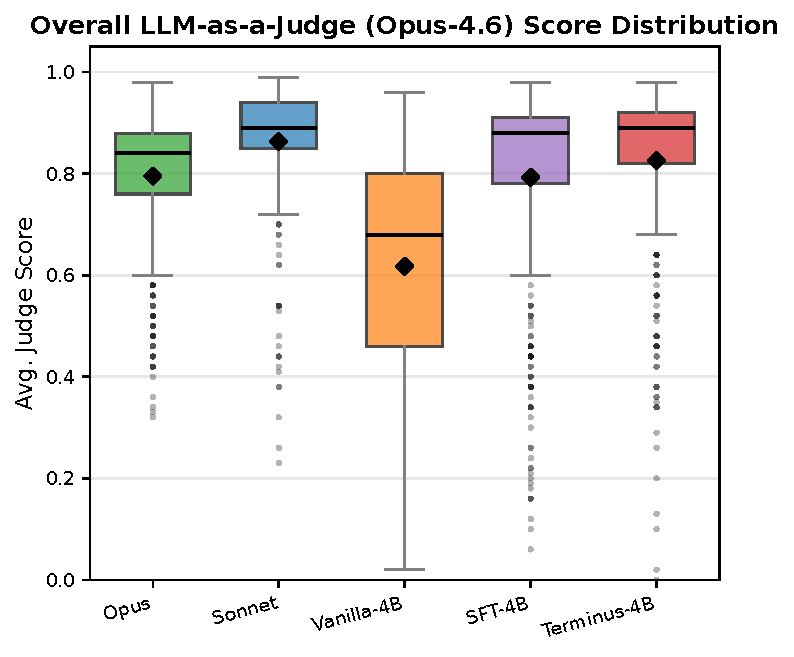
\includegraphics[width=0.95\columnwidth]{figures/judge_scores.pdf}
   \caption{在“无 Terminal”消融中，从主智能体视角评估子智能体响应质量的 LLM 评审得分。展示不同子智能体模型的总体得分分布。}
   \label{judge_scores}
\end{figure}

\subsubsection{通过 LLM 评审评价响应质量}
为了从主智能体视角衡量子智能体响应的效用，我们还采用 LLM-as-a-Judge 评估。使用 Claude Opus-4.6 作为评审模型，并提示其在给定调用子智能体前的轨迹和之后主智能体轨迹中 $N$ 个步骤的条件下，对子智能体响应评分。评估中设 $N=5$，因为我们认为这足以观察主智能体能否利用该响应。评审 LLM 沿 5 个维度对响应评分（每项均在 0 到 1 之间）：
\begin{itemize}
    \item \textbf{任务完成度：}子智能体是否完整完成了被要求完成的任务？
    \item \textbf{事实准确性：}子智能体的论断是否有事实依据，还是产生了幻觉？
    \item \textbf{信息量：}响应是否含有足够细节，使主智能体无需重跑命令即可继续？
    \item \textbf{相关性：}响应是否聚焦于任务，还是在任务外做了不必要工作？
    \item \textbf{可操作性：}主智能体能否根据响应判断下一步？子智能体的输出是否可操作？
\end{itemize}

总体得分为五个维度的均值。我们在无 Terminal 工具消融运行上执行该评估。输入评审提示的信息包括：1）主智能体的系统提示和原始问题陈述；2）子智能体调用前的轨迹（先前工具调用和结果）；3）子智能体查询和响应；4）主智能体收到子智能体响应后的后续 5 轮轨迹。后续轨迹是关键，因为它使评审器能够理解主智能体如何响应子智能体响应，以及主智能体能否直接使用它，还是必须使用不同查询重新调用子智能体。

观察结果可见，Terminus-4B 获得与前沿 LLM 相当的分数。有趣的是，Sonnet 在该评估中表现最佳。Terminus-4B 的结果似乎接近 Sonnet，并略优于 Opus。这与该配置下 Opus 和 Terminus-4B 的子$\to$子不信任指标相等（见表~\ref{swebcs_no_terminal}）相互印证。

具体比较小模型的分数，可以清楚看到 Terminus-4B 的中位数得分高于 SFT-4B。SFT 和 Terminus-4B 均优于 Vanilla 模型，表明后训练的两个阶段都很重要。

\section{局限性}
尽管结果表明，微调小语言模型能够在编码智能体的终端执行任务中有效替代前沿 LLM，仍存在若干局限：

\textbf{平台 / Shell 覆盖。}
训练和评估均偏向基于 Unix / Bash 的终端任务。尽管 Windows 上的 Powershell 或 Command Prompt、以及 Mac 上的 Zsh 在真实开发中十分常见，我们没有纳入这些 shell 的任务。将 Terminus-4B 扩展到处理这些 shell，是自然的未来研究方向。

\textbf{评估范围。}
评估几乎完全在 SWE-Bench 风格基准上完成：问题来自 GitHub issue，智能体在已包含项目所需依赖的 Docker 容器中解决它们。虽然这与文献中的先前编码智能体评估一致，却未必反映更为复杂、混乱的真实智能体使用场景；后者可能涵盖从调试应用到部署或基础设施层任务的各种工作。

\textbf{基础模型选择。}
我们只在 Qwen3-4B 模型上训练，它对该任务而言是合理的模型大小和模型族选择。结果表明，经过充分训练的 40 亿参数模型可以胜任该任务，但研究没有涵盖更大模型（8B、30B 等）及其他模型家族。相同后训练配方能否有效迁移到其他模型族 / 模型规模，仍有待验证。

\section{结论}
本文提出执行子智能体和 Terminus-4B：一个经过微调、用于在编码智能体中担任执行子智能体的 40 亿参数语言模型。通过两阶段后训练流水线，我们证明，即使是小语言模型也能在终端执行这一小而明确的任务上匹配或超过前沿 LLM 的性能，同时\textbf{将前沿 LLM 词元用量最高降低约 $\sim$30\%}。在 SWE-Bench Pro、SWE-Bench C\# 等基准上的全面评估显示，Terminus-4B 可泛化到不同编程语言，以及 Claude 和 GPT 两个常用模型家族中的不同主智能体选择。评估中的行为指标确认，后训练相较原始模型（Qwen3-4B）有显著改进，主智能体对 Terminus-4B 响应的依赖程度达到前沿 LLM 水平，很少需要重新执行工作。更广泛地说，本文展示了一种实用范式：将更小的 LM 训练为子智能体，以将词元用量转移给子智能体，从而降低编码智能体的运行成本。子智能体架构为将复杂任务分解为不同能力模型可以共享的小型子任务提供了自然方法。我们相信，结果可直接推广到其他子智能体类型，并为构建能力更强、成本更低且更易访问的编码智能体提供一条可扩展路径。

\bibliographystyle{IEEEtran}
\bibliography{iclr2024_conference}

\end{document}
